\section{Introduction}

This chapter reports and analyses the experiment results from the
trading environment and learning algorithms described in Chapter 4. The
experiments examine the financial performance of the learned agents, the
effects of two state representations, and their respective reward
functions.

The experiments are structured around four questions that directly
relate to the objectives of the dissertation to increase portfolio
wealth:

\begin{enumerate}
\def\labelenumi{\arabic{enumi}.}
\item
  \textbf{Performance:} Do the learned agents outperform appropriate
  simple benchmarks on unseen data after accounting for transaction
  costs?
\item
  \textbf{Behaviour:} Do the learned agents make use of the market and
  portfolio information provided in the state representations?
\item
  \textbf{State representation:} Does adding the drawdown feature to the
  main nine-feature state affect the learned behaviour or financial
  performance?
\item
  \textbf{Reward:} Does the risk-aware reward improve the balance
  between return and drawdown, rather than simply encouraging the agent
  to trade less?
\end{enumerate}

A key part of the analysis is determining whether the learned strategies
outperform simple strategies. Buy-and-hold, for example, is an important
benchmark here. A learned agent producing a positive return does not
necessarily indicate that it has learned a useful trading strategy if a
simple investment strategy achieves a similar or better result.

For this reason, the analysis considers both \textbf{financial
performance} and \textbf{agent behaviour}. Financial performance is
evaluated using measures including wealth change, exposure, trading
activity, drawdown, and Sharpe ratio. Behavioural analysis examines
whether an agent\textquotesingle s actions change as the state changes.
This helps to identify a policy that responds to state information
rather than one that follows a fixed trading pattern.

\section{Experiment Protocols and Evaluation Criteria}

This section describes how the experiments in this chapter were
conducted and how the reported results should be interpreted.

\subsection{Experimental Configurations}

Each configuration trained REINFORCE, Deep Q-learning (DQN), and
Proximal Policy Optimisation (PPO) separately for 80,000 steps per seed
in the portfolio environment,

To account for randomness in reinforcement learning~\cite{henderson2018}, six random seeds
were used, with an initial capital of \(C_{0} = \$ 10,000\) at the start
of every monthly episode. This means six independent training runs all
with the same configuration, allowing us to analyse the consistency of
each algorithm's results rather than relying on a single training run.

During evaluation, all policies acted deterministically: policy-gradient
algorithms select the action with the highest probability, while
value-based algorithms select the action with the highest estimated
value.

The 2023 validation period was used to make every experimental decision
reported in this chapter. This included selecting the trade size in
Section 5.3, the risk-penalty weight in Section 5.7, and the transaction
fee in Section 5.8. These choices were fixed before using them for the
main experiments in the 24 held-out test months from 2024--2025.

There are three main learned experiments in this chapter:

\begin{itemize}
\item
  The primary experiment evaluating the nine-feature state with the
  wealth-change reward.
\item
  The ten-feature state that adds drawdown while keeping the same
  wealth-change reward.
\item
  The third experiment using the ten-feature state with the risk-aware
  reward, which actually requires drawdown.
\end{itemize}

\subsection{Evaluation Metrics}

There are five financial measures used in each experiment report. They
are averaged over the episodes and, for learned agents, across the six
training seeds:

\begin{itemize}
\item
  Mean wealth change \((\Delta W)\) reported in dollars per month;
\item
  Mean exposure \((\Delta v_{t})\), which represents the proportion of
  initial capital invested in the asset and is averaged across trading
  days;
\item
  Trades per month;
\item
  Mean episode drawdown \((\Delta{dd}_{t})\);
\item
  and the monthly Sharpe ratio~\cite{sharpe1994}, a financial metric that calculates the
  average return relative to the variation of those daily returns during
  the month.
\end{itemize}

The tables also report the \textbf{seed spread}, which is the difference
between the best and worst result across the six seeds. This is included
because there might be large differences between training runs which the
average alone may hide~\cite{henderson2018}. A large spread indicates that the algorithm did
not produce a consistent trading behaviour across the different runs.

Financial performance is then followed by a behavioural analysis, as
returns alone cannot show whether a policy actually used the information
in its state. For example, a policy that buys simply because buying is
allowed can perform well during a rising market without responding to
any market information.

This led to \textbf{state-dependence analysis,} which was used to test
whether a policy\textquotesingle s actions changed when its observed
state changed while the valid actions remained the same. For instance,
if a policy selected different actions at different steps with the same
actions available, the difference could be attributed to the observed
state. The tables report how many of the six seeds met this condition.

\subsection{Benchmark Strategies}

Two non-learning strategies are used as benchmarks. They use the same
trading environment, portfolio conditions, and transaction fees as the
learned agents.

\textbf{Buy-and-hold} invests the full initial capital on the first
trading day and holds the position until the end of the month, when the
position is closed. This is the main benchmark as it is a simple passive
investment strategy.

\textbf{Always-buy} \(\mathbf{(0.25}\mathbf{C}_{\mathbf{0}}\mathbf{)}\)
purchases a fixed trade amount equal to 25\% of the initial capital
whenever buying is available, continuing until it has fully invested in
that asset. This strategy is useful for comparing against policies that
achieve their returns through repeated buying rather than by using
information from its observed state, as it also does not use any market
or portfolio information when deciding whether to buy.

\section{Fixed Trade Size Tuning}

Before comparing the learned agents with the benchmarks, the fixed
transaction size used by the learning agents must be finalized.
Determining this trading-action size matters because the amount traded
at each decision point determines how quickly the agent can build or
reduce its position during a monthly episode.

In the trading environment, each Buy or Sell action changes the trade by
a fixed fraction of the initial capital. A smaller value gives the agent
finer control over its position but also means that more trading
decisions are needed to reach a high level of asset exposure. A larger
value lets the agent build its position more quickly but provides less
control over the size of each change.

This creates a problem between the learned agents and the buy-and-hold
benchmark. Buy-and-hold invests the available capital at the beginning
of the episode, while a trading agent must build its position through
repeated actions. If the trade size uses a small, fixed transaction
size, the agent will need several trading days to reach a similar
exposure as buy-and-hold and may not overall reach the same exposure
within a typical month. Poor results could therefore arise from the
fixed trade amounts rather than from the learned policy.

The trade size was therefore calibrated using the validation data to
select the most stable size before running the main comparison between
learning algorithms on the held-out data.

\subsection{Exposure available under different transaction sizes}

The validation experiment measures the maximum exposure reachable during
a month using a policy that always buys whenever the action is
available, for each fixed transaction size. The validation set contains
12 monthly episodes, with an average length of approximately 20.8
trading days. Table 5.1 and Figure 5.1 show the results.

\addcontentsline{lot}{table}{\protect\numberline{5.1}{Attainable exposure for each fixed trade amount on the validation months. The policy buys whenever a purchase is valid.}}
\emph{Table 5.1: Attainable exposure for each fixed trade amount on the
validation months. The policy buys whenever a purchase is valid.}

{\def\LTcaptype{none} % do not increment counter
\begin{longtable}[]{@{}
  >{\centering\arraybackslash}p{(\linewidth - 6\tabcolsep) * \real{0.1725}}
  >{\centering\arraybackslash}p{(\linewidth - 6\tabcolsep) * \real{0.3929}}
  >{\centering\arraybackslash}p{(\linewidth - 6\tabcolsep) * \real{0.2374}}
  >{\centering\arraybackslash}p{(\linewidth - 6\tabcolsep) * \real{0.1973}}@{}}
\toprule\noalign{}
\begin{minipage}[b]{\linewidth}\centering
\textbf{Trade amount}
\end{minipage} & \begin{minipage}[b]{\linewidth}\centering
\textbf{Buys Days required to purchase a full asset}
\end{minipage} & \begin{minipage}[b]{\linewidth}\centering
\textbf{Mean maximum exposure}
\end{minipage} & \begin{minipage}[b]{\linewidth}\centering
\textbf{Mean wealth change}
\end{minipage} \\
\midrule\noalign{}
\endhead
\bottomrule\noalign{}
\endlastfoot
0.05C₀ & 20 & 0.450 & +\$95.49 \\
\rowsep
0.10C₀ & 10 & 0.690 & +\$121.79 \\
\rowsep
0.25C₀ & 4 & 0.838 & +\$167.39 \\
\rowsep
0.50C₀ & 2 & 0.886 & +\$162.77 \\
\rowsep
Buy-and-hold & --- & 0.910 & +\$166.92 \\
\end{longtable}
}

\begin{figure}[!htb]
  \centering
  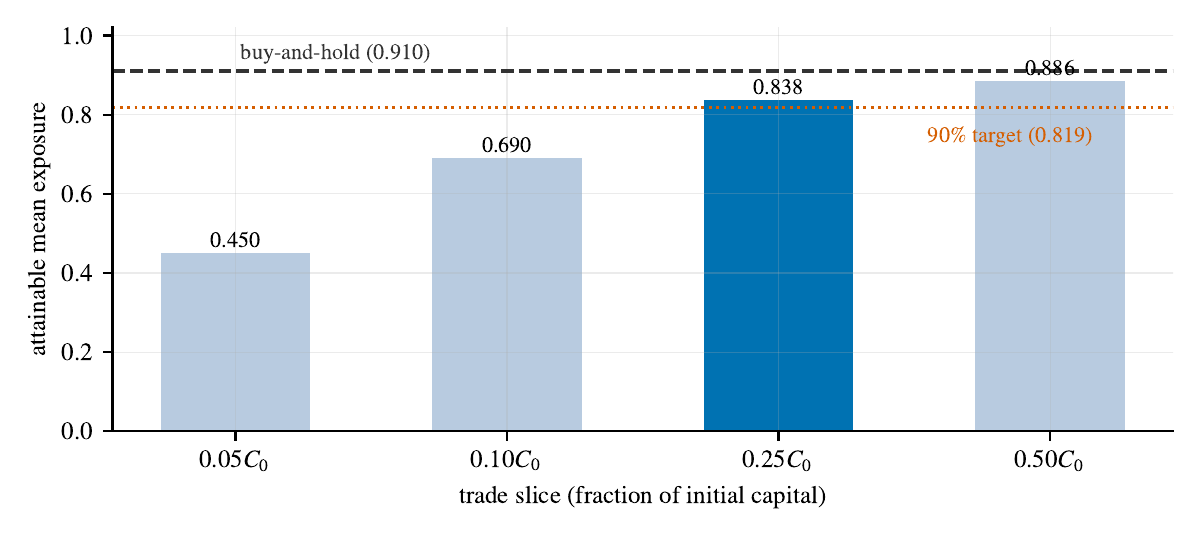
\includegraphics[width=0.9\textwidth]{media4/media/image3.png}
  \caption[Exposure ceilings from Table 5.1.]{Exposure ceilings from Table 5.1. The 0.25 C₀ trade amount (highlighted) is the smallest that clears the 90\% target of buy-and-hold's exposure; the 0.10 C₀ amount cannot reach it even in principle.}
\end{figure}


The results show that the original\(\ 0.10C₀\) trade size restricts the
agent\textquotesingle s asset exposure. This trade size requires ten buy
days to fully invest in that asset, but the average episode is only 20.8
trading days long, so half a typical month passes before full investment
is even possible.~ Its mean maximum exposure is 0.690, which is also
significantly below the 0.910 asset exposure for the simple buy-and-hold
strategy.

Hence, even a policy that buys whenever possible cannot reach the same
level of exposure as a simple benchmark during a typical monthly
episode. This matters when analysing the agent's performance. A low
return may result from poor decision-making, but it may also result from
the trading size preventing the agent from investing enough in the
asset. The two outcomes should be treated distinctly.

The \(\ 0.25C₀\) trade size was therefore selected as the primary
configuration, reaching 0.838 exposure, which corresponds to
approximately 92\% of the buy-and-hold exposure. This selection was
based on the criteria that exposure must reach at least 90\% of the
buy-and-hold, since no trade size can reach that level completely.

The buy-and-hold exposure of 0.910 gives an average exposure of
approximately 0.819 under this criterion. The \(0.25C₀\) trade size
therefore satisfies the requirement as the smallest tested trade size
whose exposure is close to the benchmark.

Increasing the trade size setting to \(0.50C₀\) raises exposure
slightly, from 0.838 to 0.886, but makes each individual action much
larger, giving the agent less control over gradual exposure changes.

Based on this calibration, the \(0.25C₀\) size balances maximum asset
exposure and control over position changes. It gives the learned agents
a reasonable opportunity to reach the benchmark level without using a
much coarser \(0.50C₀\) trade size.

\section{Do the Learned Policies Use Their Observations?}

The Financial performance of the portfolio trading agent on its own does
not show whether a learned agent is actually using the information
contained in its state representation. For example, an agent that buys
whenever buying is possible can perform well in a rising market without
using any of the market information its state provides.

This requires examining the behavioural patterns of the agents' learned
strategies to identify whether a policy selects a different action when
the state changes, provided the available valid actions remain the same.
This shows that the policy responds to its observed state rather than
simply following action constraints and can be classified as
\textbf{state-dependent.}

The experiment is performed on the validation data using the calibrated
\(0.25C₀\) trade size decided in Section 5.3, with the nine-feature
state and the primary wealth-change reward. This test aims only to
analyse behavioural differences between the algorithms by determining
whether changes in the information provided to the agent are reflected
in its decisions. It is not used to determine the final financial
performance of the agents.

Every cell was trained from scratch for this study: six seeds per
method, 80,000 steps each.

\subsection{Behaviour of the learned policies}

\addcontentsline{lot}{table}{\protect\numberline{5.2}{Behavioural Results on the validation months (0.25 C₀ trade size, nine-feature state, wealth-change reward, six freshly trained seeds). The always-buy strategy shows the maximum asset exposure this trade size can reach.}}
\emph{Table 5.2: Behavioural Results on the validation months (0.25 C₀
trade size, nine-feature state, wealth-change reward, six freshly
trained seeds). The always-buy strategy shows the maximum asset exposure
this trade size can reach.}

{\def\LTcaptype{none} % do not increment counter
\begin{longtable}[]{@{}
  >{\raggedright\arraybackslash}p{(\linewidth - 10\tabcolsep) * \real{0.1676}}
  >{\centering\arraybackslash}p{(\linewidth - 10\tabcolsep) * \real{0.1665}}
  >{\centering\arraybackslash}p{(\linewidth - 10\tabcolsep) * \real{0.1664}}
  >{\centering\arraybackslash}p{(\linewidth - 10\tabcolsep) * \real{0.1666}}
  >{\centering\arraybackslash}p{(\linewidth - 10\tabcolsep) * \real{0.1663}}
  >{\centering\arraybackslash}p{(\linewidth - 10\tabcolsep) * \real{0.1667}}@{}}
\toprule\noalign{}
\begin{minipage}[b]{\linewidth}\centering
\textbf{Policy}
\end{minipage} & \begin{minipage}[b]{\linewidth}\centering
\textbf{Mean ΔW}
\end{minipage} & \begin{minipage}[b]{\linewidth}\centering
\textbf{Seed spread}
\end{minipage} & \begin{minipage}[b]{\linewidth}\centering
\textbf{Exposure}
\end{minipage} & \begin{minipage}[b]{\linewidth}\centering
\textbf{Trades}
\end{minipage} & \begin{minipage}[b]{\linewidth}\centering
\textbf{State-dependent}
\end{minipage} \\
\midrule\noalign{}
\endhead
\bottomrule\noalign{}
\endlastfoot
\textbf{Always-buy} & +\$167.39 & --- & 0.838 & --- & --- \\
\rowsep
\textbf{REINFORCE} & +\$154.96 & \$37.29 & 0.807 & 10.3 & 0/6 \\
\rowsep
\textbf{Deep Q-learning} & +\$86.16 & \$64.20 & 0.325 & 8.5 & 6/6 \\
\rowsep
\textbf{PPO} & +\$118.55 & \$167.39 & 0.596 & 3.7 & 0/6 \\
\end{longtable}
}

\begin{figure}[!htb]
  \centering
  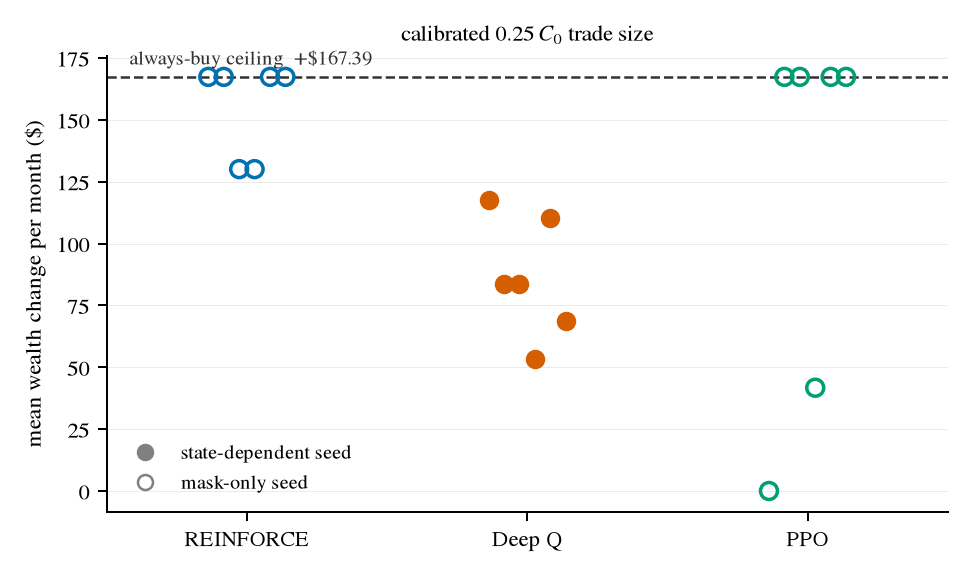
\includegraphics[width=0.9\textwidth]{media4/media/image4.png}
  \caption[Results for each seed from Table 5.2.]{Results for each seed from Table 5.2. Hollow-marker seeds show actions that don't depend on their state information; filled-marker seeds are state-dependent ones. Policy-gradient methods (REINFORCE, PPO) produce policies that cluster to either high exposure or collapse towards zero, while all six Deep Q-learning seeds fall between those corners.}
\end{figure}


Table 5.2 summarises the outcome and Figure 5.2 shows every seed
individually. The columns read as follows. Mean ΔW is the average wealth
change per month, calculated over the 12 validation months and then over
the six seeds. Seed spread is the difference between the best and worst
seeds; a spread larger than the mean produced noticeably different
results and did not agree on a strategy. State-dependent counts how many
of the six seeds act according to the experimental behaviour being
analysed.

The REINFORCE results are clearer when the individual seeds are read.
Four of its six seeds finished at exactly +\$167.39 with an exposure of
0.838. This matches the always-buy strategy, which was set as the upper
limit. These policies buy on the first four days when buying is valid,
hold the position, and close at the end of the month. The other two
seeds earned +\$130.10 while trading 20.8 times per month: Their actions
followed a fixed pattern of trading on each bar rather than changing in
response to the market state.

PPO produced three different behaviours across its six seeds. Four seeds
reached the always-buy result of +\$167.39. One seed never traded at
all, producing a wealth change of \$0.00 and an exposure of 0.000. The
remaining seed earned +\$41.73, relying on only two trading styles. This
produced a seed spread of \$167.39, showing the large difference between
the strongest and weakest PPO runs.

Deep Q-learning is the only method where none of its seeds reached
either extreme behaviours, unlike the policy-gradient methods. Its
results ranged from +\$53.23 to +\$117.43, with a mean wealth change of
+\$86.16 and an average exposure of 0.325, less than half the 0.838
standard exposure of the always-buy strategy.

\subsection{State-dependence analysis}

The final column in Table 5.2 summarises the state-dependence test, with
the count representing the difference in behaviour across the six seeds

For REINFORCE, the result of 0/6 means that none of the six
independently trained policies changed their action when the state
changed while the same actions remained valid. The four seeds that
reached the maximum exposure followed the same basic rule of buying
whenever possible, while the other two followed a fixed trading pattern.
The diagnostic therefore found no evidence that these policies used
market and portfolio features to change their decisions.

Deep Q-learning produced the opposite result. All six seeds were
classified as state-dependent. Each seed selected different actions in
states where the same valid actions were available. This indicates that
the observed current state influences the decisions made by the DQN
policies.

PPO produced the same result as REINFORCE, with 0/6 state-dependent
seeds. Taken together, the splits are categorical by algorithm family
across the three methods: all six DQN seeds were state-dependent,
compared with none of the 12 policy-gradient seeds from REINFORCE and
PPO.

\subsection{Interpretation of the learned trading behaviour}

The different results across the three methods suggest that the learning
approach had a strong influence on the type of trading behaviour that
developed. REINFORCE and PPO frequently moved towards simple policies
that did not change their actions in response to the observed state,
whereas Deep Q-learning showed state-dependent behaviour across all six
seeds.

One possible explanation is the difference between policy-gradient and
value-based learning. REINFORCE updates the probability of an action
according to the return that follows it. When the market generally
favours holding an asset, repeatedly buying can produce a strong return
without needing to sample other policies. The learning signal may
therefore settle on a simple high-exposure strategy for higher rewards
rather than exploring.

PPO uses a different update rule from REINFORCE, but it still learns a
policy directly. Its clipped objective prevents large policy changes,
which can make learning more stable, but it does not need the policy to
become state-dependent. If a simple trading rule produces consistently
positive returns, the policy may face little pressure to learn a more
complex relationship between state and action. The extreme seed outcomes
are what hint at this. Seeds from both policy-gradient methods finish at
the always-buy upper limit, since that is the most rewarding.

Deep Q-learning learns differently. Rather than adjusting action
probabilities directly, it estimates the value of each available action
in the current state and picks the action with the highest estimate at
each step. When future estimated values differ, the chosen action
changes accordingly, and the agent has to distinguish between these
actions. The state-dependent behaviour therefore becomes a structural
property of this algorithm rather than an achievement, as it necessarily
depends on the changes in the market and portfolio state.

These explanations should be treated as interpretations of observed
behaviours rather than as direct evidence of the internal learning
process. This experiment was not designed to find out the precise reason
the algorithms moved to these different strategies. They are, however,
consistent, as different seeds show that learning algorithms affect how
available state information is used to develop a trading strategy.

\section{Effect of the State Representation}

Chapter 3 defines the nine-feature state as the main state
representation used in this study. It includes market, portfolio,
position, and time information. Drawdown is intentionally treated
separately as an additional risk-related feature rather than as the last
stage of the state design.

This experiment therefore focuses on a specific question: does adding
drawdown to the nine-feature state produce a meaningful change in
performance or behaviour when the reward function remains unchanged?

The comparison keeps the following conditions fixed:

\begin{itemize}
\item
  The same wealth-change reward;
\item
  the same \(0.25C₀\) trade size;
\item
  the same held-out test period;
\item
  the same six random seeds.
\end{itemize}

The intended difference between the two configurations is therefore only
the inclusion of drawdown in the state.

\subsection{Nine-Feature vs Ten-Feature State}

{\def\LTcaptype{none} % do not increment counter
\begin{longtable}[]{@{}
  >{\raggedright\arraybackslash}p{(\linewidth - 16\tabcolsep) * \real{0.1541}}
  >{\centering\arraybackslash}p{(\linewidth - 16\tabcolsep) * \real{0.1241}}
  >{\centering\arraybackslash}p{(\linewidth - 16\tabcolsep) * \real{0.1018}}
  >{\centering\arraybackslash}p{(\linewidth - 16\tabcolsep) * \real{0.0952}}
  >{\centering\arraybackslash}p{(\linewidth - 16\tabcolsep) * \real{0.1213}}
  >{\centering\arraybackslash}p{(\linewidth - 16\tabcolsep) * \real{0.0890}}
  >{\centering\arraybackslash}p{(\linewidth - 16\tabcolsep) * \real{0.0876}}
  >{\centering\arraybackslash}p{(\linewidth - 16\tabcolsep) * \real{0.0952}}
  >{\centering\arraybackslash}p{(\linewidth - 16\tabcolsep) * \real{0.1318}}@{}}
\toprule\noalign{}
\begin{minipage}[b]{\linewidth}\centering
\textbf{Method}
\end{minipage} & \begin{minipage}[b]{\linewidth}\centering
\textbf{State}
\end{minipage} & \begin{minipage}[b]{\linewidth}\centering
\textbf{ΔW (\$)}
\end{minipage} & \begin{minipage}[b]{\linewidth}\centering
\textbf{Spread}
\end{minipage} & \begin{minipage}[b]{\linewidth}\centering
\textbf{Exposure}
\end{minipage} & \begin{minipage}[b]{\linewidth}\centering
\textbf{Trades}
\end{minipage} & \begin{minipage}[b]{\linewidth}\centering
\textbf{DD}
\end{minipage} & \begin{minipage}[b]{\linewidth}\centering
\textbf{Sharpe}
\end{minipage} & \begin{minipage}[b]{\linewidth}\centering
\textbf{State-dep.}
\end{minipage} \\
\midrule\noalign{}
\endhead
\bottomrule\noalign{}
\endlastfoot
\textbf{REINFORCE} & 9-feature & +171.51 & 24.7 & 0.810 & 10.3 & 0.0266
& 0.675 & 0/6 \\
\rowsep
\textbf{REINFORCE} & 10-feature & +167.39 & 24.7 & 0.794 & 13.0 & 0.0263
& 0.670 & 0/6 \\
\rowsep
\textbf{Deep Q} & 9-feature & +74.68 & 71.4 & 0.312 & 8.2 & 0.0124 &
0.507 & 6/6 \\
\rowsep
\textbf{Deep Q} & 10-feature & +77.81 & 89.5 & 0.354 & 7.4 & 0.0140 &
0.505 & 6/6 \\
\rowsep
\textbf{PPO} & 9-feature & +127.35 & 179.8 & 0.598 & 3.7 & 0.0195 &
0.562 & 0/6 \\
\rowsep
\textbf{PPO} & 10-feature & +159.97 & 94.0 & 0.759 & 7.3 & 0.0250 &
0.671 & 1/6 \\
\end{longtable}
}

\addcontentsline{lot}{table}{\protect\numberline{5.3}{Results of the nine- and ten-feature states on the test data (wealth-change reward, 0.25 C₀ trade size, six seeds). DD shows the mean drawdown within each episode, while State-dep. shows the number of seeds where actions changed with the observed state.}}
\emph{Table 5.3: Results of the nine- and ten-feature states on the test
data (wealth-change reward, 0.25 C₀ trade size, six seeds). DD shows the
mean drawdown within each episode, while State-dep. shows the number of
seeds where actions changed with the observed state.}

The effect of adding drawdown and the changes in mean wealth performance
for REINFORCE and DQN are small.

For REINFORCE, wealth change falls from \$171.5 with the nine-feature
state to +\$167.39 with the ten-feature state. The difference is only
−\$4.12 per month against a seed spread of \$24.70 for both
configurations, which is considerably larger than the mean wealth
change.

The behavioural result also remains unchanged. None of the six seeds are
classified as state-dependent in either configuration. Adding drawdown
therefore did not produce a noticeable change in the behaviour of the
REINFORCE policies.

DQN shows a small change in the opposite direction. Wealth increases
from +\$74.68 to +\$77.81, a change of +\$3.13 per month. The seed
spreads are \$71.40 and \$89.50, respectively, so the change between the
two state configurations is again much smaller than the variation across
seeds.

The behavioural result is unchanged for DQN. All six seeds remain
state-dependent with both state representations.

PPO appears to improve, from +\$127.35 to +\$159.97, gaining \$32.62.
However, the result needs to be considered alongside the variation
between seeds. The nine-feature configuration has a spread of
\$179.80---larger than the mean itself --- but it narrows to \$94.00 in
the ten-feature configuration, with only one seed becoming
state-dependent.

The change in the mean is therefore not enough, on its own, to show that
adding drawdown caused the improvement.

\subsection{Analysis When Drawdown Was Added}

The other performance measures columns tell the same story in different
parts. For DQN, average exposure rose from 0.312 to 0.354, and mean
drawdown from 0.0124 to 0.0140 after adding that feature to the state
--- return, exposure, and risk all moved up together by similar
proportions. Its Sharpe ratio, however, changes very little, from 0.507
to 0.505.

The patterns noticed here suggest the additional drawdown feature did
not lead to more effective risk-aware decisions, but to slightly larger
asset exposure

The changes for REINFORCE barely move. Exposure falls from 0.810 to
0.794, while drawdown decreases slightly from 0.0266 to 0.0263, as
expected of a policy algorithm that does not read the state it is given.

The small changes in the financial measures therefore do not indicate a
change in the basic policy behaviour.

Overall, the results do not show a consistent improvement in either
performance or behaviour from adding drawdown to the state while using
the default wealth-change reward.

\subsection{Interpretation}

These results do not mean that drawdown information is unimportant. They
show that, in this environment, without changing the reward objective,
the additional information did not provide a clear advantage--- an agent
maximising wealth change in general rising markets has little use for
its own loss history.

This matters because Chapter 3 introduced drawdown to provide
information that could support risk-sensitive decisions. However, this
feature becomes relevant only when the agent's learning objective makes
larger drawdowns costly while increasing portfolio wealth, which is
precisely what the risk-aware reward experiment in Section 5.7 tests.

\section{Held-Out Test Results}

The main performance question of how each learned strategy, in its final
configuration, compares with the simple benchmarks on unseen data is
evaluated on the 24 held-out months from January 2024 to December 2025.

At this point, the main configuration has been fixed:

\begin{itemize}
\item
  nine-feature state;
\item
  wealth-change reward;
\item
  \(0.25C₀\) trade size;
\item
  0.05\% transaction fee;
\item
  six random seeds.
\end{itemize}

\subsection{Overall Comparison with the Benchmark Strategies}

{\def\LTcaptype{none} % do not increment counter
\begin{longtable}[]{@{}
  >{\raggedright\arraybackslash}p{(\linewidth - 14\tabcolsep) * \real{0.1676}}
  >{\centering\arraybackslash}p{(\linewidth - 14\tabcolsep) * \real{0.1210}}
  >{\centering\arraybackslash}p{(\linewidth - 14\tabcolsep) * \real{0.1177}}
  >{\centering\arraybackslash}p{(\linewidth - 14\tabcolsep) * \real{0.1364}}
  >{\centering\arraybackslash}p{(\linewidth - 14\tabcolsep) * \real{0.1146}}
  >{\centering\arraybackslash}p{(\linewidth - 14\tabcolsep) * \real{0.1139}}
  >{\centering\arraybackslash}p{(\linewidth - 14\tabcolsep) * \real{0.1177}}
  >{\centering\arraybackslash}p{(\linewidth - 14\tabcolsep) * \real{0.1111}}@{}}
\toprule\noalign{}
\begin{minipage}[b]{\linewidth}\centering
\textbf{Policy}
\end{minipage} & \begin{minipage}[b]{\linewidth}\centering
\textbf{ΔW (\$)}
\end{minipage} & \begin{minipage}[b]{\linewidth}\centering
\textbf{Spread}
\end{minipage} & \begin{minipage}[b]{\linewidth}\centering
\textbf{Exposure}
\end{minipage} & \begin{minipage}[b]{\linewidth}\centering
\textbf{Trades}
\end{minipage} & \begin{minipage}[b]{\linewidth}\centering
\textbf{DD}
\end{minipage} & \begin{minipage}[b]{\linewidth}\centering
\textbf{Sharpe}
\end{minipage} & \begin{minipage}[b]{\linewidth}\centering
\textbf{State-dep.}
\end{minipage} \\
\midrule\noalign{}
\endhead
\bottomrule\noalign{}
\endlastfoot
\textbf{Buy-and-hold} & +180.25 & --- & 0.913 & 2.0 & 0.0310 & 0.638 &
--- \\
\rowsep
\textbf{Always-buy (}\(\mathbf{0.25}\mathbf{C₀}\)\textbf{)} & +179.75 &
--- & 0.841 & 5.0 & 0.0274 & 0.684 & --- \\
\rowsep
\textbf{REINFORCE} & +171.51 & 24.7 & 0.810 & 10.3 & 0.0266 & 0.675 &
0/6 \\
\rowsep
\textbf{Deep Q-learning} & +74.68 & 71.4 & 0.312 & 8.2 & 0.0124 & 0.507
& 6/6 \\
\rowsep
\textbf{PPO} & +127.35 & 179.8 & 0.598 & 3.7 & 0.0195 & 0.562 & 0/6 \\
\end{longtable}
}

\addcontentsline{lot}{table}{\protect\numberline{5.4}{test results over the 24 held-out months (2024--2025): benchmarks and the three learned agents in their final configuration, six seeds each.}}
\emph{Table 5.4: test results over the 24 held-out months (2024--2025):
benchmarks and the three learned agents in their final configuration,
six seeds each.}

Table 5.4 is the central result of this dissertation.

Two simple strategies are used as benchmarks. Buy-and-hold invests the
full capital on the first day and is the benchmark an investor would
actually compare against. Always-buy at \(0.25C₀\) buys an asset at a
quarter fraction of the initial capital. This takes trades with every
valid action until it has fully invested in the asset. It represents a
strategy that buys unconditionally at the fixed trade size, without
requiring observations.

The central result is straightforward: none of the three learned agents
outperformed buy-and-hold during the held-out test period.

Buy-and-hold earned +\$180.25 per month, equivalent to a 1.8025\%
increase of the initial capital per monthly episode, and no learned
agent reached this. The closest was REINFORCE at +\$171.51, which was
\$8.74 short of buy-and-hold per month; PPO earned +\$127.35 and Deep
Q-learning +\$74.68.

Always buying at \(0.25C₀\) earned +\$179.75, within \$0.50 of
buy-and-hold, and it sets the standard a learned agent must reach/beat
before it can claim any skill, as matching it needs no market
information at all --- only buying whenever buying is available.

\begin{figure}[!htb]
  \centering
  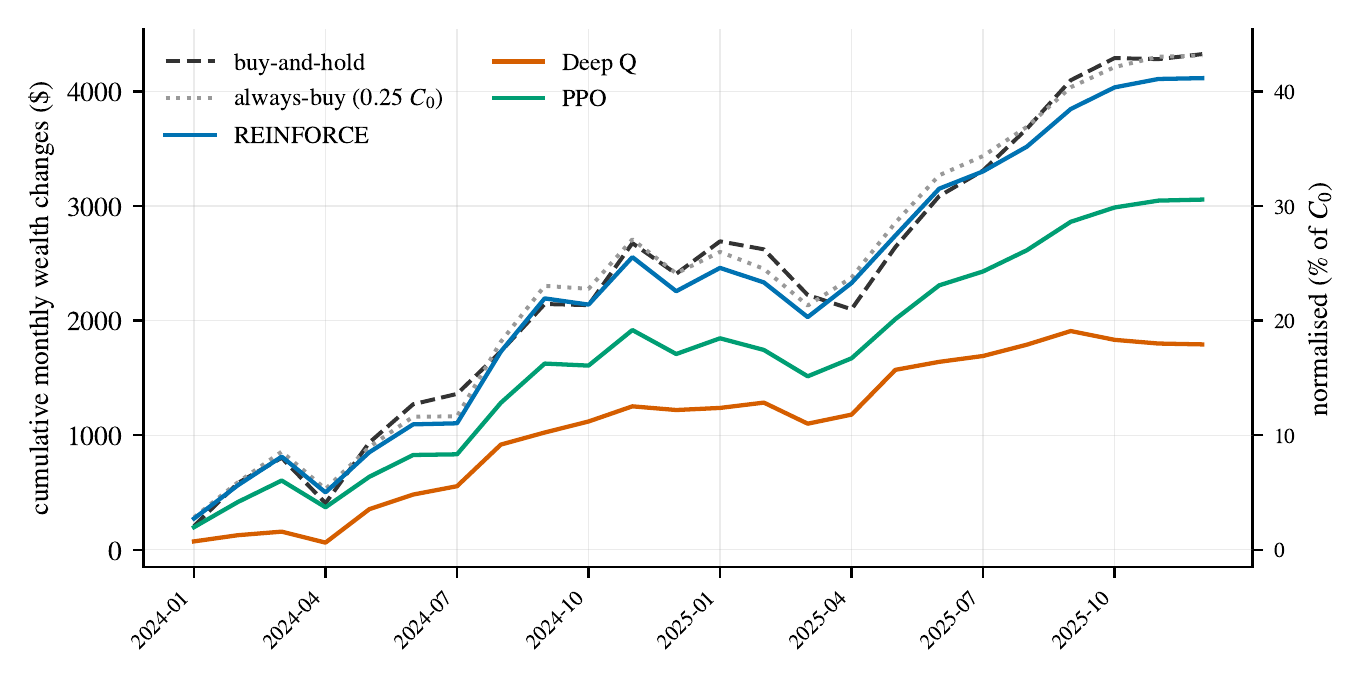
\includegraphics[width=0.9\textwidth]{media4/media/image5.png}
  \caption[Cumulative sum of average monthly wealth changes across the test months.]{Cumulative sum of average monthly wealth changes across the test months. Each monthly episode resets to C₀, so the lines show the sum of monthly gains and losses rather than compound; the right axis expresses percentages of initial capital C₀. REINFORCE follows Always-buy (0.25 C₀) and buy-and-hold almost exactly, while Deep Q-learning shows a flatter line due to low exposure, including through the March--April 2025 decline.}
\end{figure}


Over the full two years, the gap compounds visibly in Figure 5.3:
buy-and-hold accumulates to +\$4,326 in monthly wealth change at the end
of 2025, REINFORCE to +\$4,116 closely following buy-and-hold, PPO to
+\$3,056, and Deep Q-learning at the lowest value of +\$1,792.

\subsection{Return and market exposure}

The exposure column explains most of the return column. The REINFORCE
result is particularly interesting; its return was close to buy-and-hold
at +\$171.51. Its average exposure was 0.810, compared with 0.913 for
buy-and-hold, and none of its six seeds were state-dependent, suggesting
the high return came mainly from staying invested rather than learning
when to enter or leave the market. Its behaviour was therefore closer to
the Always-buy at \(0.25C\) accumulation strategy. Hence why it sits
within a few percent of Always-buy results (+\$179.75, exposure 0.841).

DQN produced a different result. All six seeds were state-dependent,
showing that the agent changed its actions in response to state
information, and chose to participate the least, with the lowest
exposure of 0.312 and a wealth change of \$74.68. These results are
roughly a third of the buy-and-hold benchmarks, so the lower return may
therefore be correlated with reduced market participation.

PPO produced a return between REINFORCE and DQN, with an average wealth
change of \$127.35 and exposure of 0.598. However, its seed spread was
179.8, which is larger than its mean return. This shows that the six PPO
runs produced different outcomes and should not be treated as a single
stable trading strategy.

\subsection{Risk and risk-adjusted performance}

Lower returns can still be desirable if they follow a sufficient
reduction in risk. For this reason, drawdown and Sharpe ratio are also
used alongside return. Figure 5.4 puts every learned configuration in
this chapter on that scale.

\begin{figure}[!htb]
  \centering
  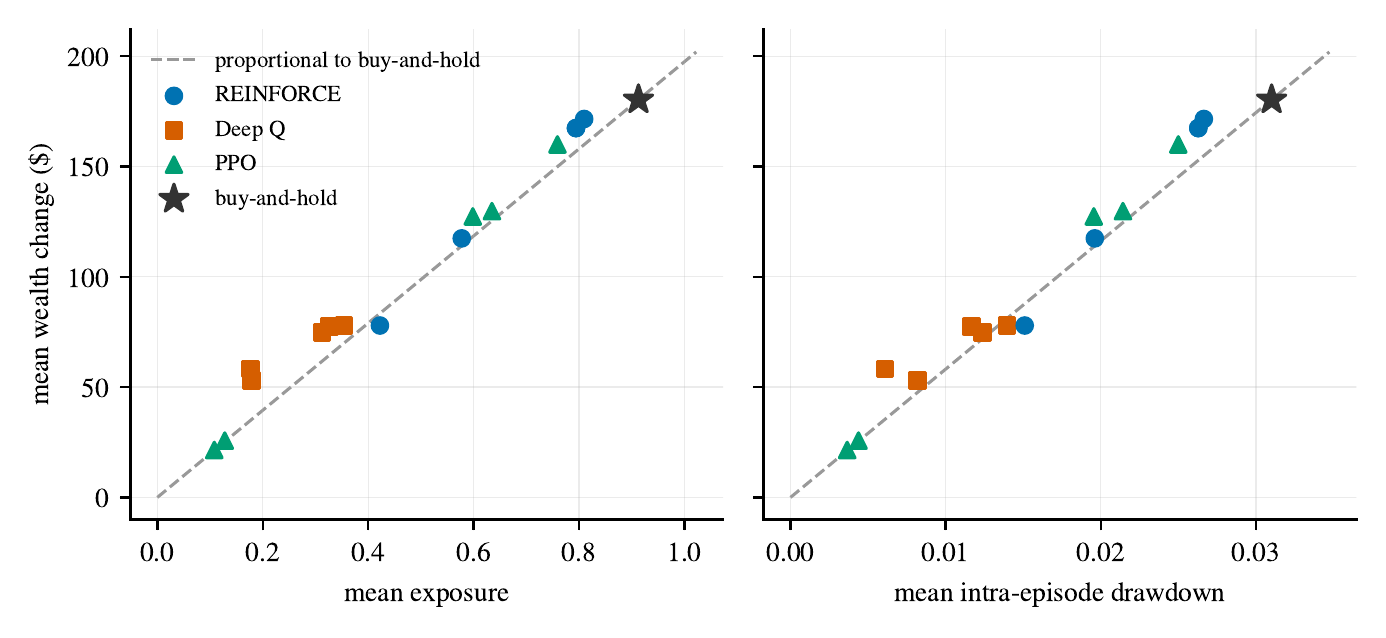
\includegraphics[width=0.9\textwidth]{media4/media/image6.png}
  \caption[Average wealth change compared with exposure (left) and daily drawdown (right) for every learned configuration in this chapter.]{Average wealth change compared with exposure (left) and daily drawdown (right) for every learned configuration in this chapter. The dashed lines show the proportional relationship with buy-and-hold. None of the learned configurations show a clear improvement over either line.}
\end{figure}


Buy-and-hold earned \$197 per unit of exposure. An agent that merely
holds less of the same asset lands on the dashed proportional line;
genuine downside management would appear above it.

Deep Q-learning is an informative case. It earned 41.4\% of the
buy-and-hold benchmark's return at 34.2\% of its exposure (0.312) and
40.0\% of its drawdown (0.0124) --- return and risk fell equally, which
is more like scaling down. Its Sharpe ratio of 0.507 versus
buy-and-hold's 0.638 confirms it earned less return per unit of risk
exposed to, not more.

The results therefore do not indicate that DQN achieved better
risk-adjusted performance than the benchmark. Its lower drawdown largely
came from lower exposure, not from a strategy that intentionally avoided
the market\textquotesingle s decline periods.

\subsection{Behaviour During the March 2025 Decline}

March 2025 provides a useful example because it was the worst test month
for the buy-and-hold benchmark. During this month, buy-and-hold lost
\$398.41, i.e. 3.9841\% of the initial capital, with a drawdown of
approximately 5.6\%. If the state-dependent agent, Deep Q-learning, had
recognised the conditions, this would have been the month to step aside.
Instead, DQN had a mean exposure of 0.490 in March--- higher than its
overall average exposure of 0.312 for the entire test period--- and lost
\$184.04, 46\% of the benchmark's loss.

These results are important when interpreting the state-dependence
finding. Even in a month when reducing exposure before the decline could
have helped, it did not significantly reduce exposure, and these March
2025 losses match its equivalent market participation. Hence, its lower
drawdown cannot be attributed to knowing when to avoid bad market
periods, but to holding less overall.

\begin{figure}[!htb]
  \centering
  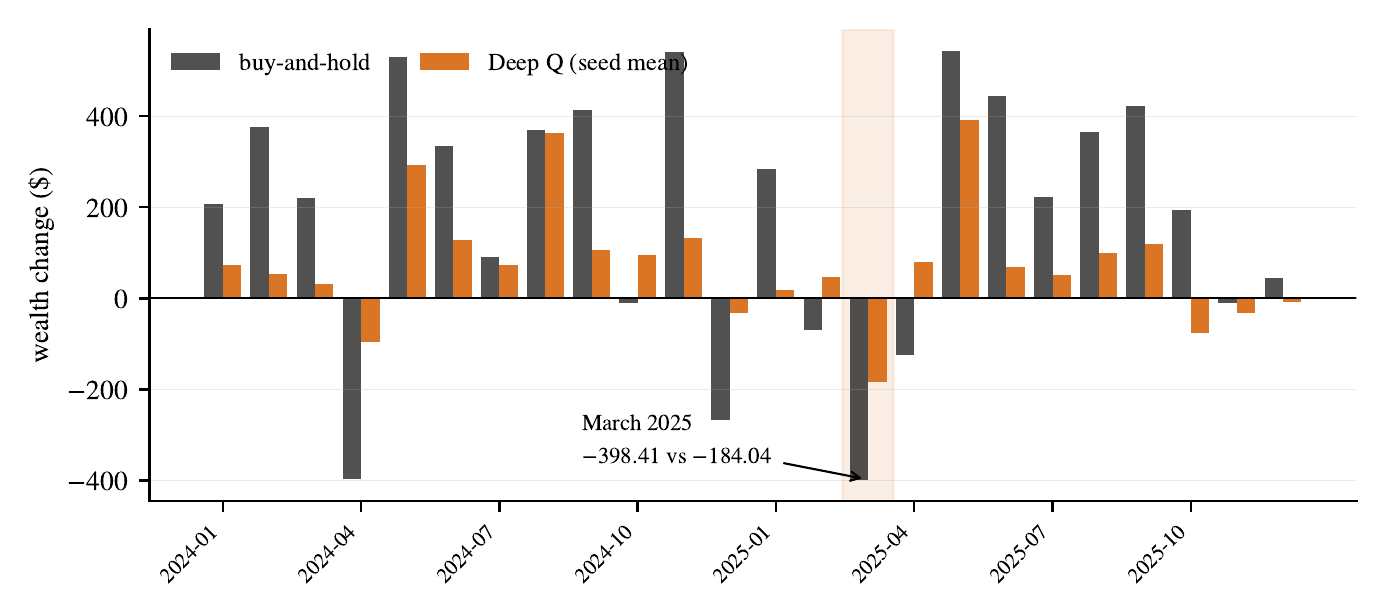
\includegraphics[width=0.9\textwidth]{media4/media/image7.png}
  \caption[Monthly wealth changes of buy-and-hold and Deep Q-learning over the 24 test months.]{Monthly wealth changes of buy-and-hold and Deep Q-learning over the 24 test months. The agent's bars match a 1/3 scaling of the benchmark's bars in almost every month: In March 2025, the worst month, it lost \$184.04 compared to the benchmark's \$398.41 loss.}
\end{figure}


Figure 5.5 extends to all 24 months. Each pair of bars is one test
month: the dark bar represents buy-and-hold's wealth change, and the
orange bar represents the Deep Q-learning for the same month. The two
series appear to rise and fall together --- the agent's best month is
the benchmark's best month (May 2025, +\$390.80 compared to +\$543.11)
and its worst is the benchmark's worst (the discussed March 2025).

Buy-and-hold lost money in seven of the 24 months, and the agent ended
positive in three of those seven. Those three months, however, produced
little profit compared to the benchmark losses

In the two heavy down months, April 2024 (−\$396.08) and March 2025
(−\$398.41), the agent was also at a loss---approximately 24\% and 46\%
of the benchmark's loss, respectively---correlating to its 34\% average
market participation and one-third scaling to the benchmark. Where
drawdown management mattered most, the agent still left the position
open to losses.

\subsection{Trading behaviour and Seed consistency}

The results also show considerable differences in consistency between
the algorithms. To examine this, we analyse seed spreads, which measure
differences between runs.

REINFORCE had the smallest seed spread (\$24.70), showing seeds agree
with each other. However, this consistency should be interpreted with
its behavioural results. All six seeds were classified as
state-independent and exhibited similar behaviour, precisely because
they agree on ignoring market information and generally being highly
exposed, as that is more rewarding. The small spread therefore does not
necessarily indicate that REINFORCE learned a more reliable trading
strategy.

DQN had a larger spread of \$71.40. This is consistent with the six
seeds learning different state-dependent policies, resulting in greater
variations in their returns.

PPO had the largest spread of \$179.80, which was greater than the mean
return, also showing that individual seeds ranged from near-inactivity
to near-full investment in Fig. 5.2, and none were state-dependent.

These results show why evaluating a single random seed would not provide
enough evidence for a reliable conclusion about the learning algorithms.
Behaviour and performance can vary considerably from one training run to
the next.

\section{Effect of the Risk-Aware Reward}

Earlier experiments showed that the main wealth-change reward did not
always encourage agents to respond differently to changes in the
observed state. It simply rewards changes in portfolio wealth.

Chapter 3.5 identifies the limitation of this objective: it does not
penalize large portfolio drawdowns, raising the question of whether
explicitly including portfolio drawdown in the reward would lead to more
risk-aware behaviour.

To examine this, the risk-aware reward was introduced in which it was
modified to include a penalty for increases in drawdown:

\[r_{t}^{risk} = \Delta W_{t} - \lambda C_{0}\Delta dd_{t}.\]

where

\(\Delta dd_{t}\) is the increase in portfolio drawdown at trading day
\(t\) (and is zero when drawdown does not rise), and coefficient
\(\lambda\) controls the penalty effects. The initial capital \(C_{0}\)
factor puts \(\Delta dd_{t}\) in dollars so that 𝜆 is dimensionless.

The risk-aware reward is paired with the ten-feature state using the
drawdown feature because it provides the agent with information about
its current position relative to its previous maximum wealth.

\subsection{Selection of the Penalty size}

The penalty size was selected using the validation set and Deep
Q-learning as the selector because it is the only algorithm whose
policies consistently respond to the state (Section 5.4). The held-out
test period was not used for this decision.

A selection rule was created. The penalised configuration must keep at
least half (50\%) of both the unpenalised return---to still earn a
decent amount --- and the unpenalised exposure---to still participate in
the market.

The unpenalised DQN configuration had a mean wealth change of \$78.35
and exposure of 0.445. The resulting minimum requirements were
therefore:

\[\Delta W \geq \$ 39.17\]

and

\[Exposure \geq 0.223.\]

The results of the penalty sweep are shown in Table 5.5.

{\def\LTcaptype{none} % do not increment counter
\begin{longtable}[]{@{}
  >{\raggedright\arraybackslash}p{(\linewidth - 10\tabcolsep) * \real{0.1900}}
  >{\centering\arraybackslash}p{(\linewidth - 10\tabcolsep) * \real{0.1610}}
  >{\centering\arraybackslash}p{(\linewidth - 10\tabcolsep) * \real{0.1633}}
  >{\centering\arraybackslash}p{(\linewidth - 10\tabcolsep) * \real{0.1652}}
  >{\centering\arraybackslash}p{(\linewidth - 10\tabcolsep) * \real{0.1605}}
  >{\centering\arraybackslash}p{(\linewidth - 10\tabcolsep) * \real{0.1600}}@{}}
\toprule\noalign{}
\begin{minipage}[b]{\linewidth}\centering
\textbf{λ}
\end{minipage} & \begin{minipage}[b]{\linewidth}\centering
\textbf{Mean ΔW}
\end{minipage} & \begin{minipage}[b]{\linewidth}\centering
\textbf{Exposure}
\end{minipage} & \begin{minipage}[b]{\linewidth}\centering
\textbf{Drawdown}
\end{minipage} & \begin{minipage}[b]{\linewidth}\centering
\textbf{DD change}
\end{minipage} & \begin{minipage}[b]{\linewidth}\centering
\textbf{Passes}
\end{minipage} \\
\midrule\noalign{}
\endhead
\bottomrule\noalign{}
\endlastfoot
\textbf{0 (unpenalised)} & +\$78.35 & 0.445 & 0.0163 & --- & --- \\
\rowsep
\textbf{0.05} & +\$88.78 & 0.401 & 0.0128 & −21.5\% & yes \\
\rowsep
\textbf{0.10} & +\$67.30 & 0.344 & 0.0124 & −24.0\% & yes \\
\rowsep
\textbf{0.25} & +\$19.90 & 0.074 & 0.0035 & −78.4\% & no \\
\rowsep
\textbf{0.50} & +\$1.73 & 0.002 & 0.0001 & −99.4\% & no \\
\rowsep
\textbf{1.00} & \$0.00 & 0.000 & 0.0000 & −100\% & no \\
\rowsep
\textbf{2.00} & \$0.00 & 0.000 & 0.0000 & −100\% & no \\
\end{longtable}
}

\addcontentsline{lot}{table}{\protect\numberline{5.5}{Risk-penalty size on the validation months (Deep Q-learning, six seeds). The rule requires ΔW ≥ +\$39.17 and exposure ≥ 0.223; the largest passing value that meets both requirements is λ = 0.10.}}
\emph{Table 5.5: Risk-penalty size on the validation months (Deep
Q-learning, six seeds). The rule requires ΔW ≥ +\$39.17 and exposure ≥
0.223; the largest passing value that meets both requirements is λ =
0.10.}

\begin{figure}[!htb]
  \centering
  
\includegraphics[width=0.9\textwidth]{media5/media/image1.png}
  \caption[Results from the penalty size of Table 5.5. Left: mean wealth change against λ with the requirement floor of +\$39.17. Right: exposure and drawdown relative to their values without penalties.]{Results from the penalty size of Table 5.5. Left: mean wealth change against λ with the requirement floor of +\$39.17. Right: exposure and drawdown relative to their values without penalties. Between λ = 0.10 and 0.25, exposure drops sharply rather than decreasing gradually.}
\end{figure}


The results show a clear change in behaviour of the penalty \(\lambda\)
as the size increases. At \(\lambda = 0.10\) , the agent still maintains
a meaningful level of exposure and a return of \$67.30.

Increasing the penalty to 0.25 causes exposure to fall sharply to 0.074.
The agent loses about 78\% of its exposure, indicating reluctance to
trade. At \(\lambda = 0.50\) and above, the agent stops trading
completely.

This result depicts an important limitation of the reward formulation.
The simplest way for an agent to reduce drawdown is to hold less of the
asset or simply not hold it at all. In theory, a portfolio that remains
in cash is not exposed to asset movements and therefore does not
experience market drawdowns. Once the drawdown penalty becomes too
large, market participation becomes unattractive.

Based on these criteria, the largest coefficient that satisfied both the
return and exposure requirements was therefore:

\[\boxed{\lambda = 0.10}.
\]This became the fixed penalty value for evaluating the main risk-aware
experiment.

\subsection{Effect on the Test Set}

The selected risk-aware reward was then evaluated on the held-out test
set.

{\def\LTcaptype{none} % do not increment counter
\begin{longtable}[]{@{}
  >{\raggedright\arraybackslash}p{(\linewidth - 14\tabcolsep) * \real{0.1675}}
  >{\centering\arraybackslash}p{(\linewidth - 14\tabcolsep) * \real{0.1192}}
  >{\centering\arraybackslash}p{(\linewidth - 14\tabcolsep) * \real{0.1202}}
  >{\centering\arraybackslash}p{(\linewidth - 14\tabcolsep) * \real{0.1162}}
  >{\centering\arraybackslash}p{(\linewidth - 14\tabcolsep) * \real{0.1364}}
  >{\centering\arraybackslash}p{(\linewidth - 14\tabcolsep) * \real{0.1125}}
  >{\centering\arraybackslash}p{(\linewidth - 14\tabcolsep) * \real{0.1117}}
  >{\centering\arraybackslash}p{(\linewidth - 14\tabcolsep) * \real{0.1162}}@{}}
\toprule\noalign{}
\begin{minipage}[b]{\linewidth}\centering
\textbf{Algorithm}
\end{minipage} & \begin{minipage}[b]{\linewidth}\centering
\textbf{Reward}
\end{minipage} & \begin{minipage}[b]{\linewidth}\centering
\textbf{ΔW (\$)}
\end{minipage} & \begin{minipage}[b]{\linewidth}\centering
\textbf{Spread}
\end{minipage} & \begin{minipage}[b]{\linewidth}\centering
\textbf{Exposure}
\end{minipage} & \begin{minipage}[b]{\linewidth}\centering
\textbf{Trades}
\end{minipage} & \begin{minipage}[b]{\linewidth}\centering
\textbf{DD}
\end{minipage} & \begin{minipage}[b]{\linewidth}\centering
\textbf{Sharpe}
\end{minipage} \\
\midrule\noalign{}
\endhead
\bottomrule\noalign{}
\endlastfoot
\textbf{REINFORCE} & wealth & +167.39 & 24.7 & 0.794 & 13.0 & 0.0263 &
0.670 \\
\rowsep
\textbf{REINFORCE} & risk & +167.39 & 24.7 & 0.794 & 13.0 & 0.0263 &
0.670 \\
\rowsep
\textbf{Deep Q} & wealth & +77.81 & 89.5 & 0.354 & 7.4 & 0.0140 &
0.505 \\
\rowsep
\textbf{Deep Q} & risk & +52.90 & 43.1 & 0.178 & 5.4 & 0.0082 & 0.416 \\
\rowsep
\textbf{PPO} & wealth & +159.97 & 94.0 & 0.759 & 7.3 & 0.0250 & 0.671 \\
\rowsep
\textbf{PPO} & risk & +21.48 & 128.9 & 0.108 & 0.7 & 0.0037 & 0.107 \\
\end{longtable}
}

\addcontentsline{lot}{table}{\protect\numberline{5.6}{Wealth-change versus risk-aware reward (λ = 0.10) on the held-out months, ten-feature state, six seeds.}}
\emph{Table 5.6: Wealth-change versus risk-aware reward (λ = 0.10) on
the held-out months, ten-feature state, six seeds.}

The DQN result gives the clearest evidence of the effect of the
risk-aware reward. For Deep Q-learning, the mean drawdown falls from
0.0140 under the standard reward to 0.0082 with the risk-aware reward, a
reduction of approximately 41\%. However, its return also falls from
+\$77.81 to +\$52.90, a reduction of about 32\%. Exposure falls from
0.354 to 0.178, meaning that the agent decides to hold only half as much
of the asset.

The results do not suggest improved risk-adjusted performance. Instead,
the reward mainly encouraged the agent to reduce its exposure to the
asset, and the Sharpe ratio also decreased from 0.505 to 0.416.

The PPO results show the same effect more strongly. With the risk-aware
reward, PPO\textquotesingle s exposure fell to 0.108, and its average
trading activity dropped below one trade per month, from 7.3 to 0.7. As
a result, its mean wealth change decreased from \$159.97 to +\$21.48.

REINFORCE shows no noticeable change. Its results are identical for both
rewards. This is consistent with the earlier behavioural findings:
REINFORCE policies do not change their trading behaviour simply by
changing the reward.

\subsection{Interpretation of the risk-aware return}

The risk-aware reward changed the behaviour of the state-dependent
agents, but there is no clear evidence that it led to better risk
management. Instead, the results suggest that the penalty mainly
encouraged the agents to reduce their exposure to the asset.

These results do not show that risk-aware reinforcement learning is
ineffective in general. However, they do show a limitation of the reward
formulation used in this study. An agent's policy could reduce drawdown
to zero by simply holding less of that asset or by never entering the
market, but this would not satisfy the main objective of generating
useful investment returns.

A more effective objective would therefore need to consider both return
and risk, rather than mainly penalising exposure to drawdown. The
relevant question becomes whether the agent can \textbf{reduce drawdown
while still leading to meaningful returns and exposure.} For example,
the objective could reward the agent for achieving higher returns for a
given level of risk. Chapter 6 discusses other possible alternatives in
future work.

\section{Transaction-Fee Sizing}

Transaction costs are an important part of the trading environment
because frequent trading can reduce the returns produced by a strategy,
even when individual decisions appear reasonable. A strategy may appear
profitable before fees are included but become less attractive once the
cost of each trade is taken into account.

The main experiments use a transaction fee of 0.05\%. To test whether
the observed behaviour changes as this fee varies, the fee was swept
from 0 basis points (0.00\%) to 50basis points (0.50\%) on the
validation months with the nine-feature state, and everything else held
fixed.

The sweep was run on all algorithms, each with six freshly trained seeds
per fee level. Table 5.7 and Figure 5.7 report the outcome.

{\def\LTcaptype{none} % do not increment counter
\begin{longtable}[]{@{}
  >{\raggedright\arraybackslash}p{(\linewidth - 14\tabcolsep) * \real{0.1320}}
  >{\centering\arraybackslash}p{(\linewidth - 14\tabcolsep) * \real{0.1243}}
  >{\centering\arraybackslash}p{(\linewidth - 14\tabcolsep) * \real{0.1242}}
  >{\centering\arraybackslash}p{(\linewidth - 14\tabcolsep) * \real{0.1237}}
  >{\centering\arraybackslash}p{(\linewidth - 14\tabcolsep) * \real{0.1242}}
  >{\centering\arraybackslash}p{(\linewidth - 14\tabcolsep) * \real{0.1237}}
  >{\centering\arraybackslash}p{(\linewidth - 14\tabcolsep) * \real{0.1242}}
  >{\centering\arraybackslash}p{(\linewidth - 14\tabcolsep) * \real{0.1237}}@{}}
\toprule\noalign{}
\begin{minipage}[b]{\linewidth}\centering
\textbf{Fee}
\end{minipage} & \begin{minipage}[b]{\linewidth}\centering
\textbf{B\&H ΔW}
\end{minipage} & \begin{minipage}[b]{\linewidth}\centering
\textbf{REINF. ΔW}
\end{minipage} & \begin{minipage}[b]{\linewidth}\centering
\textbf{REINF. trades}
\end{minipage} & \begin{minipage}[b]{\linewidth}\centering
\textbf{Deep Q ΔW}
\end{minipage} & \begin{minipage}[b]{\linewidth}\centering
\textbf{Deep Q trades}
\end{minipage} & \begin{minipage}[b]{\linewidth}\centering
\textbf{PPO ΔW}
\end{minipage} & \begin{minipage}[b]{\linewidth}\centering
\textbf{PPO trades}
\end{minipage} \\
\midrule\noalign{}
\endhead
\bottomrule\noalign{}
\endlastfoot
\textbf{0bps(0.00\%)} & +\$177.09 & +\$177.56 & 5.0 & +\$108.00 & 10.9 &
+\$155.35 & 4.5 \\
\rowsep
\textbf{5bps(0.05\%)} & +\$166.92 & +\$154.96 & 10.3 & +\$86.16 & 8.5 &
+\$118.55 & 3.7 \\
\rowsep
\textbf{10bps(0.10\%)} & +\$156.76 & +\$143.74 & 4.7 & +\$77.60 & 8.9 &
+\$78.50 & 2.7 \\
\rowsep
\textbf{25bps(0.25\%)} & +\$126.33 & +\$88.76 & 10.3 & +\$32.35 & 3.9 &
+\$26.40 & 1.2 \\
\rowsep
\textbf{50bps(0.50\%)} & +\$75.83 & +\$41.31 & 2.8 & +\$16.32 & 1.9 &
+\$12.60 & 1.0 \\
\end{longtable}
}

\addcontentsline{lot}{table}{\protect\numberline{5.7}{Transaction Fee sizing on the validation months; six seeds. Trades are per month. Fees are shown in basis points and as a percentage of trade value.}}
\emph{Table 5.7: Transaction Fee sizing on the validation months; six
seeds. Trades are per month. Fees are shown in basis points and as a
percentage of trade value.}

\begin{figure}[!htb]
  \centering
  
\includegraphics[width=0.9\textwidth]{media5/media/image2.png}
  \caption{Transaction Fee sizing from Table 5.7. Left: average wealth change falls for every strategy as fees rise. Right: average trades per month as fees rise.}
\end{figure}


\subsection{Effect of transaction costs on returns \& trading behaviour}

As expected, higher transaction fees reduce the returns of the different
algorithm strategies. The effect is important for strategies that trade
frequently because more of their portfolio gains go to transaction
costs.

Deep Q-learning shows the clearest reduction in trading activity as the
fee of taking a trade increases. Its average number of trades falls from
10.9 per month at 0bps (0.00\%) to 1.9 at 50bps (0.50\%), an 83\%
reduction. As each action gets more expensive, the agent acts less,
reducing exposure. This is consistent with the algorithm correctly
incorporating transaction costs into its environment.

REINFORCE does not show the same clear pattern. Its trade counts vary,
running from 5.0, 10.3, 4.7, 10.3, and 2.8, respectively, with no
consistent decrease in trades taken as the fee rises. This aligns with
the earlier state-independent results: an agent that does not rely on
information from its current state to make decisions is less likely to
adjust its behaviour when trading costs change.

PPO's average trade count also falls from 4.5 to 1.0, showing that many
seeds are pushed to stop trading due to higher fees. This is also why
the average return collapses by 77\%, from +\$177.56 to +\$41.31, a
difference of \$136.25 per month, even though the average trade count
moves only gently.

\subsection{Interpretation}

The transaction-fee experiment therefore reflects another difference
between the learning algorithms in terms of their change in behaviour.
Deep Q-learning changes its trading behaviour as trading costs increase,
even though its overall returns are below the buy-and-hold benchmark. This mirrors the fee response reported by Th\'eate and Ernst, whose agent also traded less as the assumed costs rose~\cite{theate2021}.
REINFORCE produces returns generally closer to the buy-and-hold
strategy, and it also shows higher exposure that does not respond
consistently to changes in transaction costs. PPO, on the other hand,
shows a major collapse in returns as fees increase, while its trade
counts decline more gently. Overall, the learned agents lose
proportionally more because they trade more often in this experiment.

This indicates that the learning system is capable of responding to
different changes when the learned policy is sufficiently
state-dependent.

\section{Discussion of the Main Findings}

The experiments produced several findings about both the performance of
the learning agents and the way they behaved within the trading
environment. They also answer the research questions of Section 5.1

\subsection{The Benchmark Remains Difficult to Beat}

The main finding is that none of the learned agents could outperform the
simple buy-and-hold benchmark on the held-out test period. Buy-and-hold
achieved a wealth change of \$180.25, compared with \$171.51 for
REINFORCE as the best learned agent, while every other agent fell
further behind with \$127.35 for PPO, and \$74.68 for DQN.

However, it is important to note that the test period consists of
generally favourable market conditions. Therefore, the experiments
cannot simply be viewed as evidence that reinforcement learning failed,
as staying invested in generally rising markets is already a strong
strategy

Buy-and-hold is therefore a difficult benchmark to improve upon, which is consistent with the market-efficiency expectation set out in Chapter 2~\cite{fama1970}. A
learned strategy that reduces exposure must therefore focus on periods
when leaving the market is advantageous enough to compensate for the
return not gained while being out of the market.

The experiments provide limited evidence that the tested agents could
make this decision and overall did not demonstrate such behaviour.

\subsection{Additional State Features Did Not Lead to Better Performance}

The state comparison did not show a consistent advantage from adding
drawdown to the nine-feature state. This is important because the state
representation was designed to include information about market
movements, portfolio position, wealth, and risk.

For REINFORCE and DQN, the changes in return were -\$4.12 and \$3.13,
respectively, in the nine-to-ten-feature comparison. This does not
necessarily mean the features were poorly selected, nor that the
nine-feature state is universally sufficient. It means that, in this
particular environment and with this wealth-change objective, additional
market information produced no measurable improvement. The later
risk-aware experiments show the behaviour changing only when the
objective itself included drawdown, and mainly through reduced market
participation.

\subsection{The Algorithms Differed in Their Use of the State}

One of the clearest differences between the algorithms is behavioural
rather than financial. REINFORCE and PPO often produced policies that
were classified as state-independent, so their relatively strong returns
need careful interpretation: a policy that buys whenever possible can
perform well in rising markets without using the information provided to
it. Deep Q-learning was state-dependent in all six seeds, but its use of
the state generally reduced exposure rather than raising returns.

This is why financial return alone is not enough to evaluate the learned
policies. Without the behavioural analysis, the strong performance of
REINFORCE could be mistaken for evidence that the model had learned a
useful relationship between market information and trading decisions.

\subsection{Lower Risk Was Mainly Associated with Lower Exposure}

The results show a consistent relationship between market participation
and risk; specifically, risk was reduced mainly by participating less in
the market.

Deep Q-learning achieved lower drawdown than buy-and-hold, but this was
due to lower exposure, and overall, it led to lower returns in the same
proportion.

This means lower drawdown should not be interpreted as evidence that DQN
avoided the worst market movements, as this differs from identifying and
avoiding specific periods of downside markets.

A proper risk-management strategy would ideally remain invested during
rising market periods while reducing exposure during market downsides
once detected. The current results do not provide enough evidence to
conclude that the agent learned this type of selective risk management.

\subsection{The Trade Size Affects Performance}

The trade size experiment shows that the transaction size is part of the
problem definition rather than merely an implementation design. A small
trading size limits how much exposure an agent can build during a
monthly episode, so poor performance may stem from the trade size rather
than the quality of the learned policy. The calibration in Section 5.3
addressed this by selecting the \(0.25C_{0}\) size, which brings the
attainable exposure close to the benchmark\textquotesingle s. Notably,
changing the trade size had a larger effect on performance than adding
features to the state, which supports calibrating it before working on
the main learned strategies.

\subsection{Transaction Costs Provided a Useful Behavioural Test}

The transaction-fee experiment showed that Deep Q-learning reduced its
trading activity by approximately 83\% as the fee rose from zero to
0.50\%, while REINFORCE did not show the same response. This provides
further evidence that Deep Q-learning was making greater use of the
information available through the environment, although this additional
responsiveness did not result in better financial performance.

\subsection{Variation Between Seeds Is Important}

This experiment showed considerable variation between random seeds,
especially for the policy-gradient methods.

In some configurations, different seeds produced noticeably different
behaviours. Some policies turned towards high exposure, while others
traded less or became more conservative.

A seed producing a strong return would not be enough to conclude that
the algorithm had learned a reliable trading strategy. Consistent
behaviour across multiple seeds proves that, and becomes stronger
evidence that, the observed result is derived from that algorithm rather
than a product of one training run.

\subsection{Implications for the Research Objectives}

Overall, the experiments provide a qualified answer to the main research
question of whether reinforcement learning algorithms can learn
profitable trading strategies for a portfolio (in this case, the SPY
asset).

The reinforcement learning agents learned trading policies, but the
experiments did not show they could outperform the simpler buy-and-hold
benchmark on unseen data.

The results also show that learning behaviour strongly depends on the
algorithm, with clear differences between the learning methods.
REINFORCE moved towards remaining invested and made little use of state
information. DQN, however, consistently changed its actions based on the
observed state, making it highly state-dependent, but it did not yield
higher returns.

PPO behaviour was closer to REINFORCE than to DQN. Although PPO uses an
actor-critic structure and a clipped policy objective to stabilise
updates, its performance was less consistent across seeds, with a larger
spread in returns. This suggests that PPO\textquotesingle s additional
stability mechanisms did not produce an effective trading policy in this
environment.

The risk-aware reward also changed the behaviour of the state-dependent
agents and reduced drawdown, but the reduction was mainly due to lower
market exposure rather than better timing for entering and exiting
markets during downward periods. When the penalty became too large, the
agents almost stopped trading altogether.

These findings suggest that the main challenge identified by the
experiments is not just related to providing the agent with more
information. Instead, the results strongly point to the interaction
between the \textbf{reward function, trade size, and the behaviour
learned by the agent} as key factors in determining whether the
resulting strategy is useful.

\section{Chapter Summary}

The chapter first determines the final trade size because this affects
how quickly an agent can build or reduce its position. It then examines
whether the learned strategies rely on the information from the state
representations, followed by a comparison between the main nine-feature
state and the additional risk-aware state. It then presents the main
held-out test results, followed by experiments on the risk-aware reward
and the effect of transaction costs. The chapter concludes by bringing
the findings together and relating them to the research objectives.

The results show that none of the learned agents consistently
outperforms the buy-and-hold benchmark over the held-out dataset. The
behavioral analysis offers more insight into this outcome. The
policy-gradient algorithms rely less on available state information,
whereas the value-based agent uses more available state information but
generally has a lower exposure. The experiments also indicate that the
fixed trading amount affects performance. Finally, the drawdown-based
reward reduces both return and exposure, suggesting that the risk-aware
reward mainly encourages lower market participation rather than
generating better risk-adjusted trading performance.
